\documentclass[12pt]{report}
\usepackage[utf8]{inputenc}
\usepackage{graphicx}
\graphicspath{{img/}}
\usepackage{pdflscape}
\usepackage{afterpage}
\usepackage[table,xcdraw]{xcolor}
\usepackage{multirow}
\usepackage{minted}
\usepackage{array}
\usepackage{float}
\usepackage{amsthm}
\usepackage{amsmath}
\usepackage{setspace}



\makeatletter

\usepackage[letterpaper, margin=1in]{geometry}

\usepackage[sorting=none]{biblatex}
\addbibresource{references.bib}

\usepackage{afterpage}

\newcommand\blankpage{%
    \null
    \thispagestyle{empty}%
    \addtocounter{page}{-1}%
    \newpage}
    
%Establece el estilo de caption de tablas y figuras.
\usepackage[center,font=small,format=plain,labelfont=bf,up,textfont=it,up]{caption}
\captionsetup[figure]{labelformat=simple, labelsep=period}
\captionsetup[table]{labelformat=simple, labelsep=period}


%Establece el estilo de header y footer para todas las p�ginas de la tesis
\usepackage{fancyhdr}
\pagestyle{fancy}
\renewcommand{\chaptermark}[1]{ \markboth{\chaptername\ \thechapter.\ #1}{}}
\renewcommand{\sectionmark}[1] {\markright{\thesection.\ #1}}
\renewcommand{\headrulewidth}{0.5pt}
\renewcommand{\footrulewidth}{0pt}
\fancyhf{}
\fancyhead[LO]{\nouppercase{\leftmark}}
\fancyhead[RE]{\nouppercase{\rightmark}}
\fancyfoot[CE,CO]{\thepage}


\newcommand{\framework}{\textit{framework}}


\begin{document}

\thispagestyle{empty}
\begin{table}[H]
\begin{minipage}[t][0.8\paperheight][s]{0.08\columnwidth}%
\noindent \vspace{0cm}

\begin{flushright}
\includegraphics[scale=0.3]{img/nearsoft.png}\end{flushright}%


\end{minipage}\hfill{}%
\begin{minipage}[t][0.8\paperheight][s]{0.86\columnwidth}%
\noindent \begin{center}
\textbf{\huge{}\vspace{0cm}
Nearsoft}{\Large{}\medskip{}
}
\par\end{center}{\Large \par}

\begin{doublespace}
\noindent \begin{center}
\textbf{\Large{}Academy 2018B}
\par\end{center}{\Large \par}
\end{doublespace}

\begin{center}
\textbf{\large{}Build Something From Scratch}
\par\end{center}{\large \par}

\noindent \begin{center}
{\large{}``Vulnerability Scanner'' }
\par\end{center}{\large \par}


\noindent \begin{center}
\emph{Team members:}
\par\end{center}

\begin{onehalfspace}
\noindent \begin{center}
{\large{}Juan Daniel Amparan de la Garza}\\
{\large{}Hugo Fernando Licón Valenzuela}\\
{\large{}Guillermo Martínez Espina}\\
{\large{}Hector Manuel Robles Montes}\\
{\large{}Jose Manuel Ruiz Ruiz}\\
{\large{}Jose Francisco Saldana Ortega}\\
{\large{}Brian Harlán Samaniego Dávila}\\
{\large{}Andrés Sánchez Pérez}\\
{\large{}Javier Ivan Venegas Carrillo}
\par\end{center}{\large \par}

\end{onehalfspace}


\noindent \begin{center}
{\large{}}
\par\end{center}{\large \par}

\noindent \begin{flushright}
{\large{}\vspace{7mm}
}{\small{}CDMX,  \today.}
\par\end{flushright}%
\end{minipage}
\end{table}



%\chapter*{Dedicatoria}
%\afterpage{\blankpage}
%\chapter{Agradecimientos}
%\afterpage{\blankpage}

\tableofcontents
\listoffigures
%\listoftables




\chapter{Introduction}
Users trust web services with sensitive information, like credit card information,  birthdays, and addresses. This makes Web Applications a high-value target for bad intentioned folks also known as Black Hat Hackers.

It is the duty of the service provider to assure that the user information will be secure, this responsibility ends up in the hands of the developers.

This tool aims to help developers safeguard their Web Applications and Services providing a vulnerability scanner that can be used to find well known security holes.

It is designed to find various vulnerabilities using "black-box" method, that means it won't study the source code of web applications but will work using fuzz testing, scanning the pages of the deployed web application, extracting links and forms and attacking the scripts.

\section{What?}

The objective of this project is to deliver a web platform where users can check if a web page has ten of the Web Application Security Risks, by providing and scanning the url of the web page. The platform will contain a dashboard for the user, where it will show the scans results, represented by graphs and text, and also the user will have the option to export the report in .PDF, .XML and .TXT formats, or keep consulting it at the web platform by logging with his user account \cite{owasp}.

\section{Why?}
The importance of delivering a web platform that can scan the security risks of other web platforms, is to have a powerful tool that can be used for testing new websites and verify if a website is exposed to the most common security risks.


\section{How?}
The software will have several components, it will connect to Python REST API to perform certain tasks to test web vulnerabilities that could take a lot of time to finish.The application itself will be developed using Ruby On Rails, Python and PostgreSQL to manage data.

\section{Limitations}
Due to the time and the way some vulnerabilities checks have to be done (access to the website’s source code and/or the server), we consider that it is not feasible to implement some vulnerabilities or to extend the functionality of the already implemented ones.

\section{Vulnerabilities}
The vulnerabilities tested by this application are the following ones: 

\begin{itemize}
    \item XSS - Cross Site Scripting
    \item DOM based XSS
    \item Blind SQL Injection
    \item SQL Injection
    \item HTTP Header SQL Injection
    \item PHP Injection
    \item OS Command Injection
    \item HTML Injection
    \item XML Injection 
    \item LDAP Injection
\end{itemize}




\chapter{Design}

In this chapter the approach for building the application will be shown with different diagrams and as well some diagrams which could help the understanding of the application's flow. 


\section{C4 Modeling}

First of all for the sake of simplicity and understanding the design will be explained using the C4 model architecture. 

As shown in the Figure \ref{fig:c41}, a System Context diagram is shown and it allows to step back and see the big picture of the application.

\begin{figure}[h!]
    \centering
    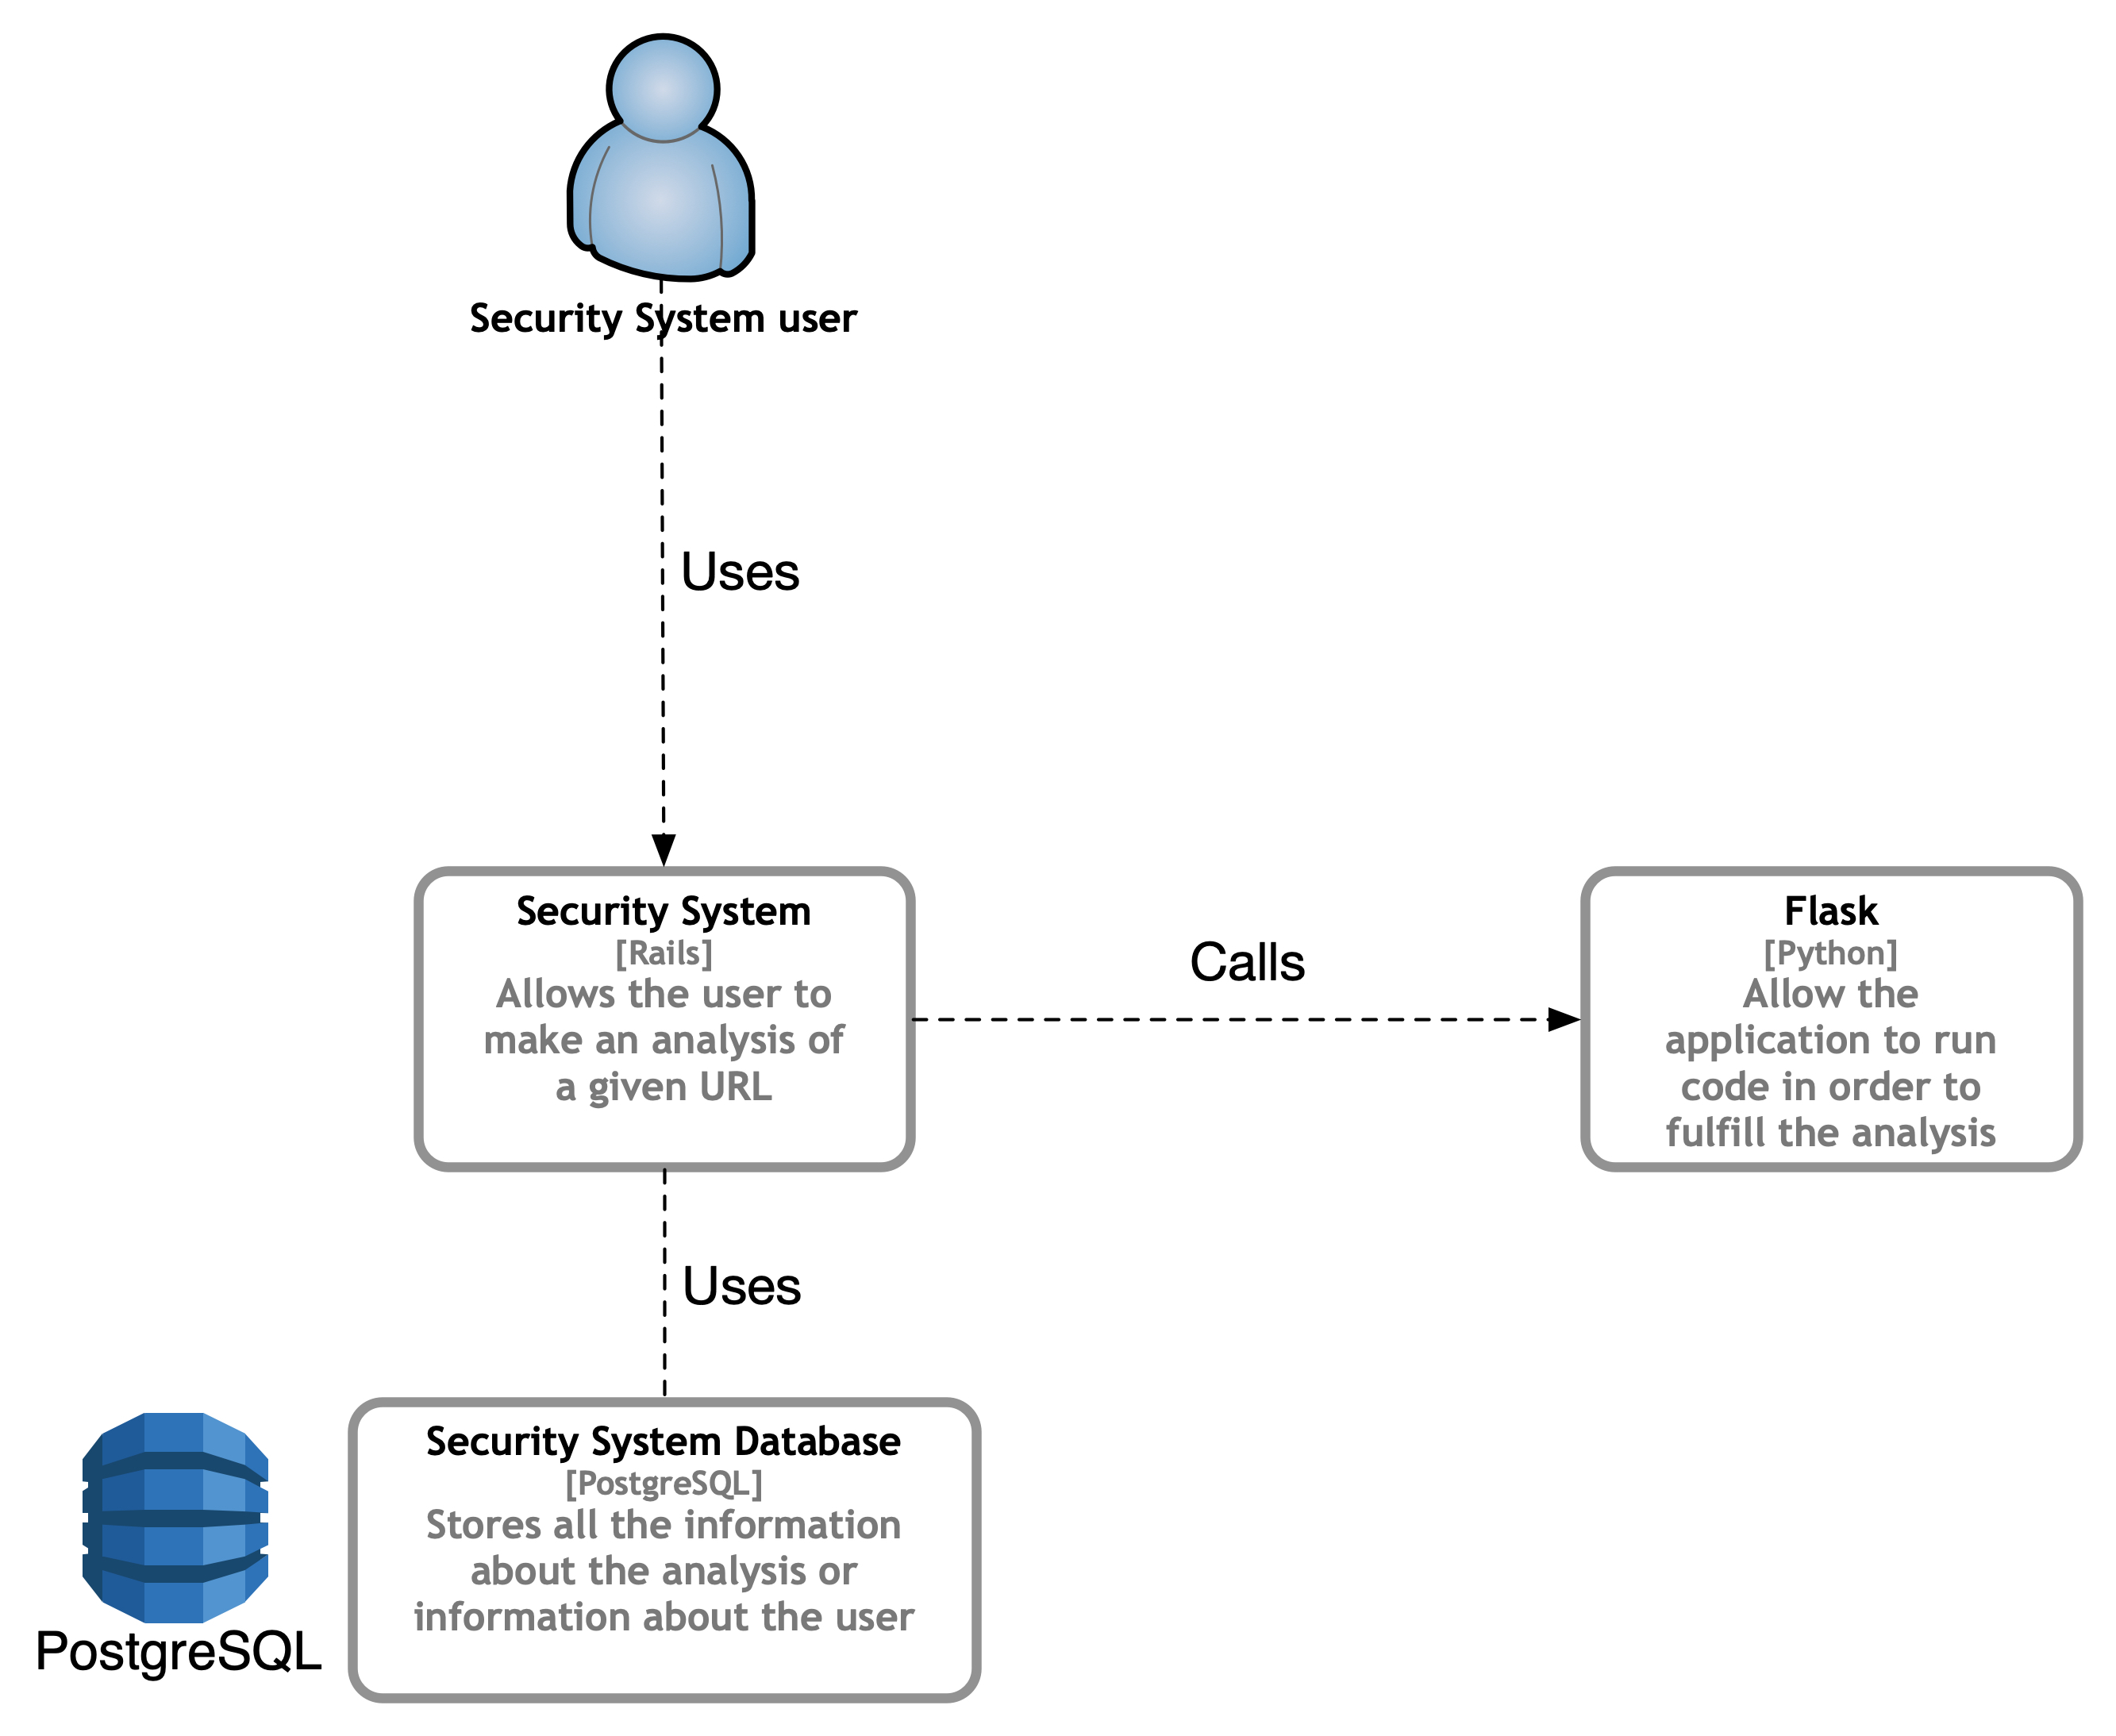
\includegraphics[width=10cm]{img/C41.jpg}
    \caption{System Context diagram}
    \label{fig:c41}
\end{figure}

\clearpage

In the Figure \ref{fig:c42} the Container Diagram helps explaining the system in a deeper overview than the System Context Diagram. The Container diagram shows the high-level shape of the software architecture and how responsibilities are distributed across it. It also shows the major technology choices and how the containers communicate with one another \cite{c4model}.

\begin{figure}[h!]
    \centering
    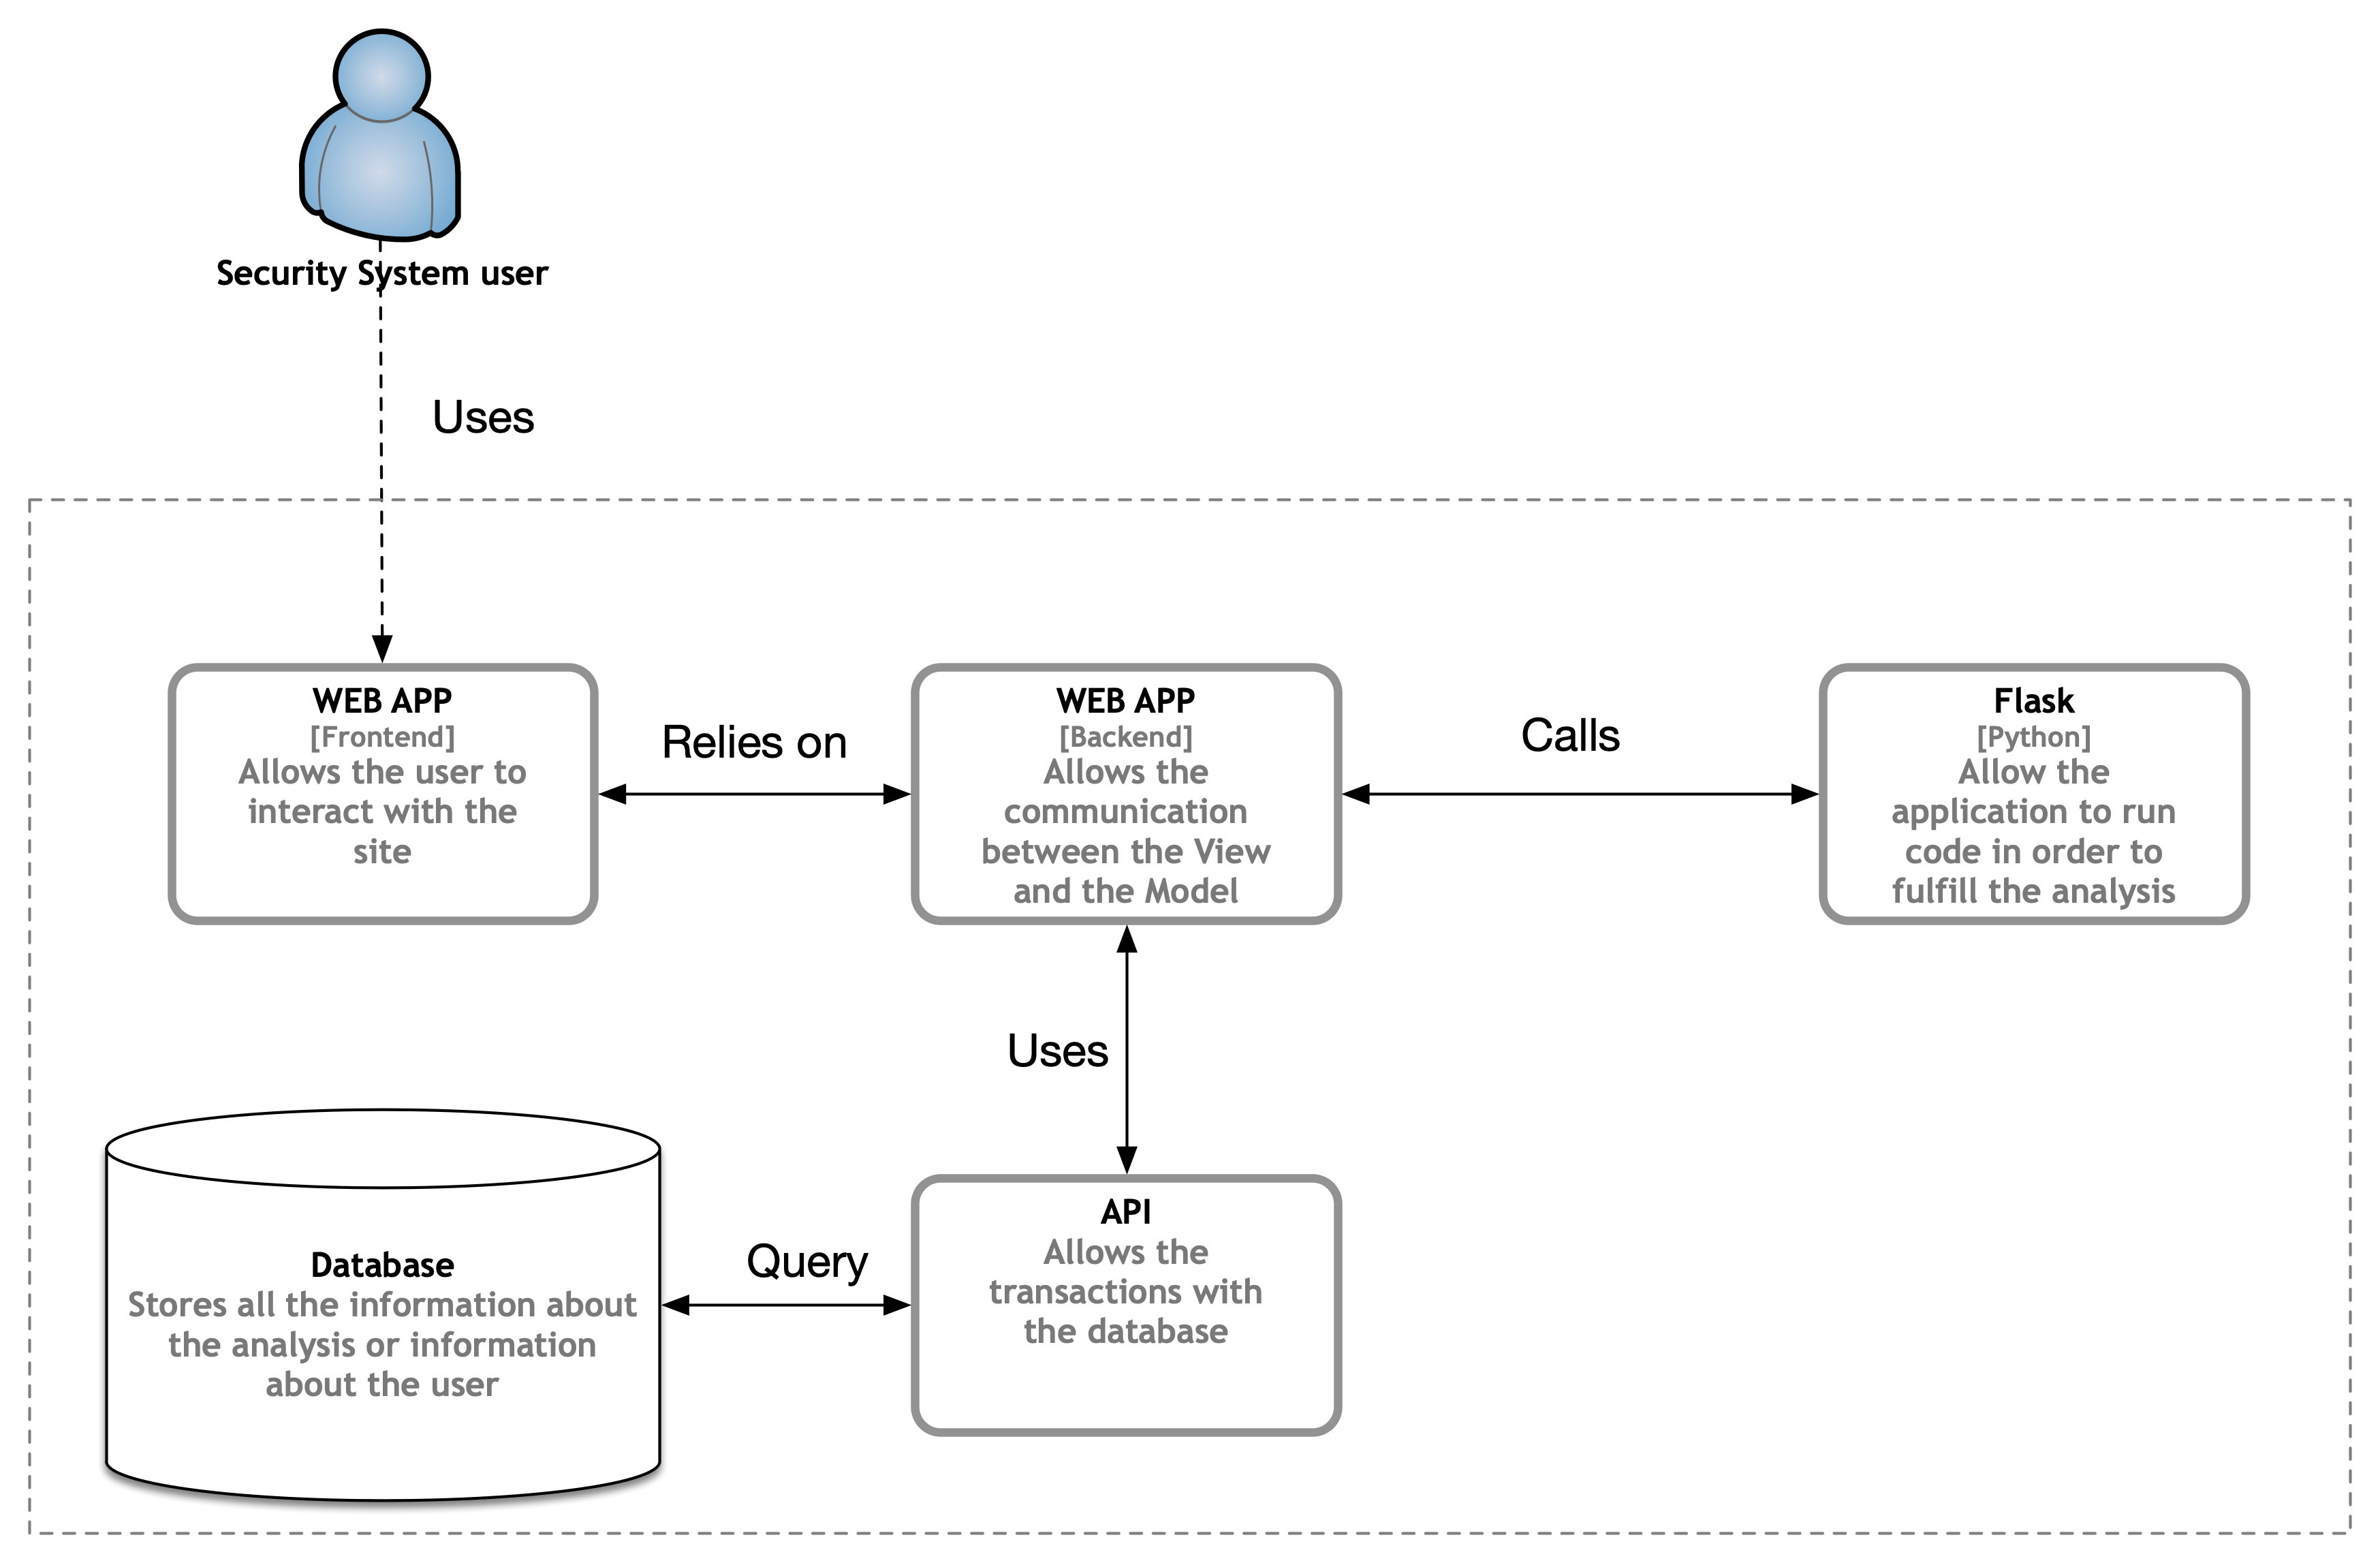
\includegraphics[width=14cm]{img/C42.jpg}
    \caption{Container diagram}
    \label{fig:c42}
\end{figure}

\clearpage

Finally on the Component diagram we identify the major structural building blocks and their interactions, it shows the different components of the application, their responsibilities and the technology/implementation details.

\begin{figure}[h!]
    \centering
    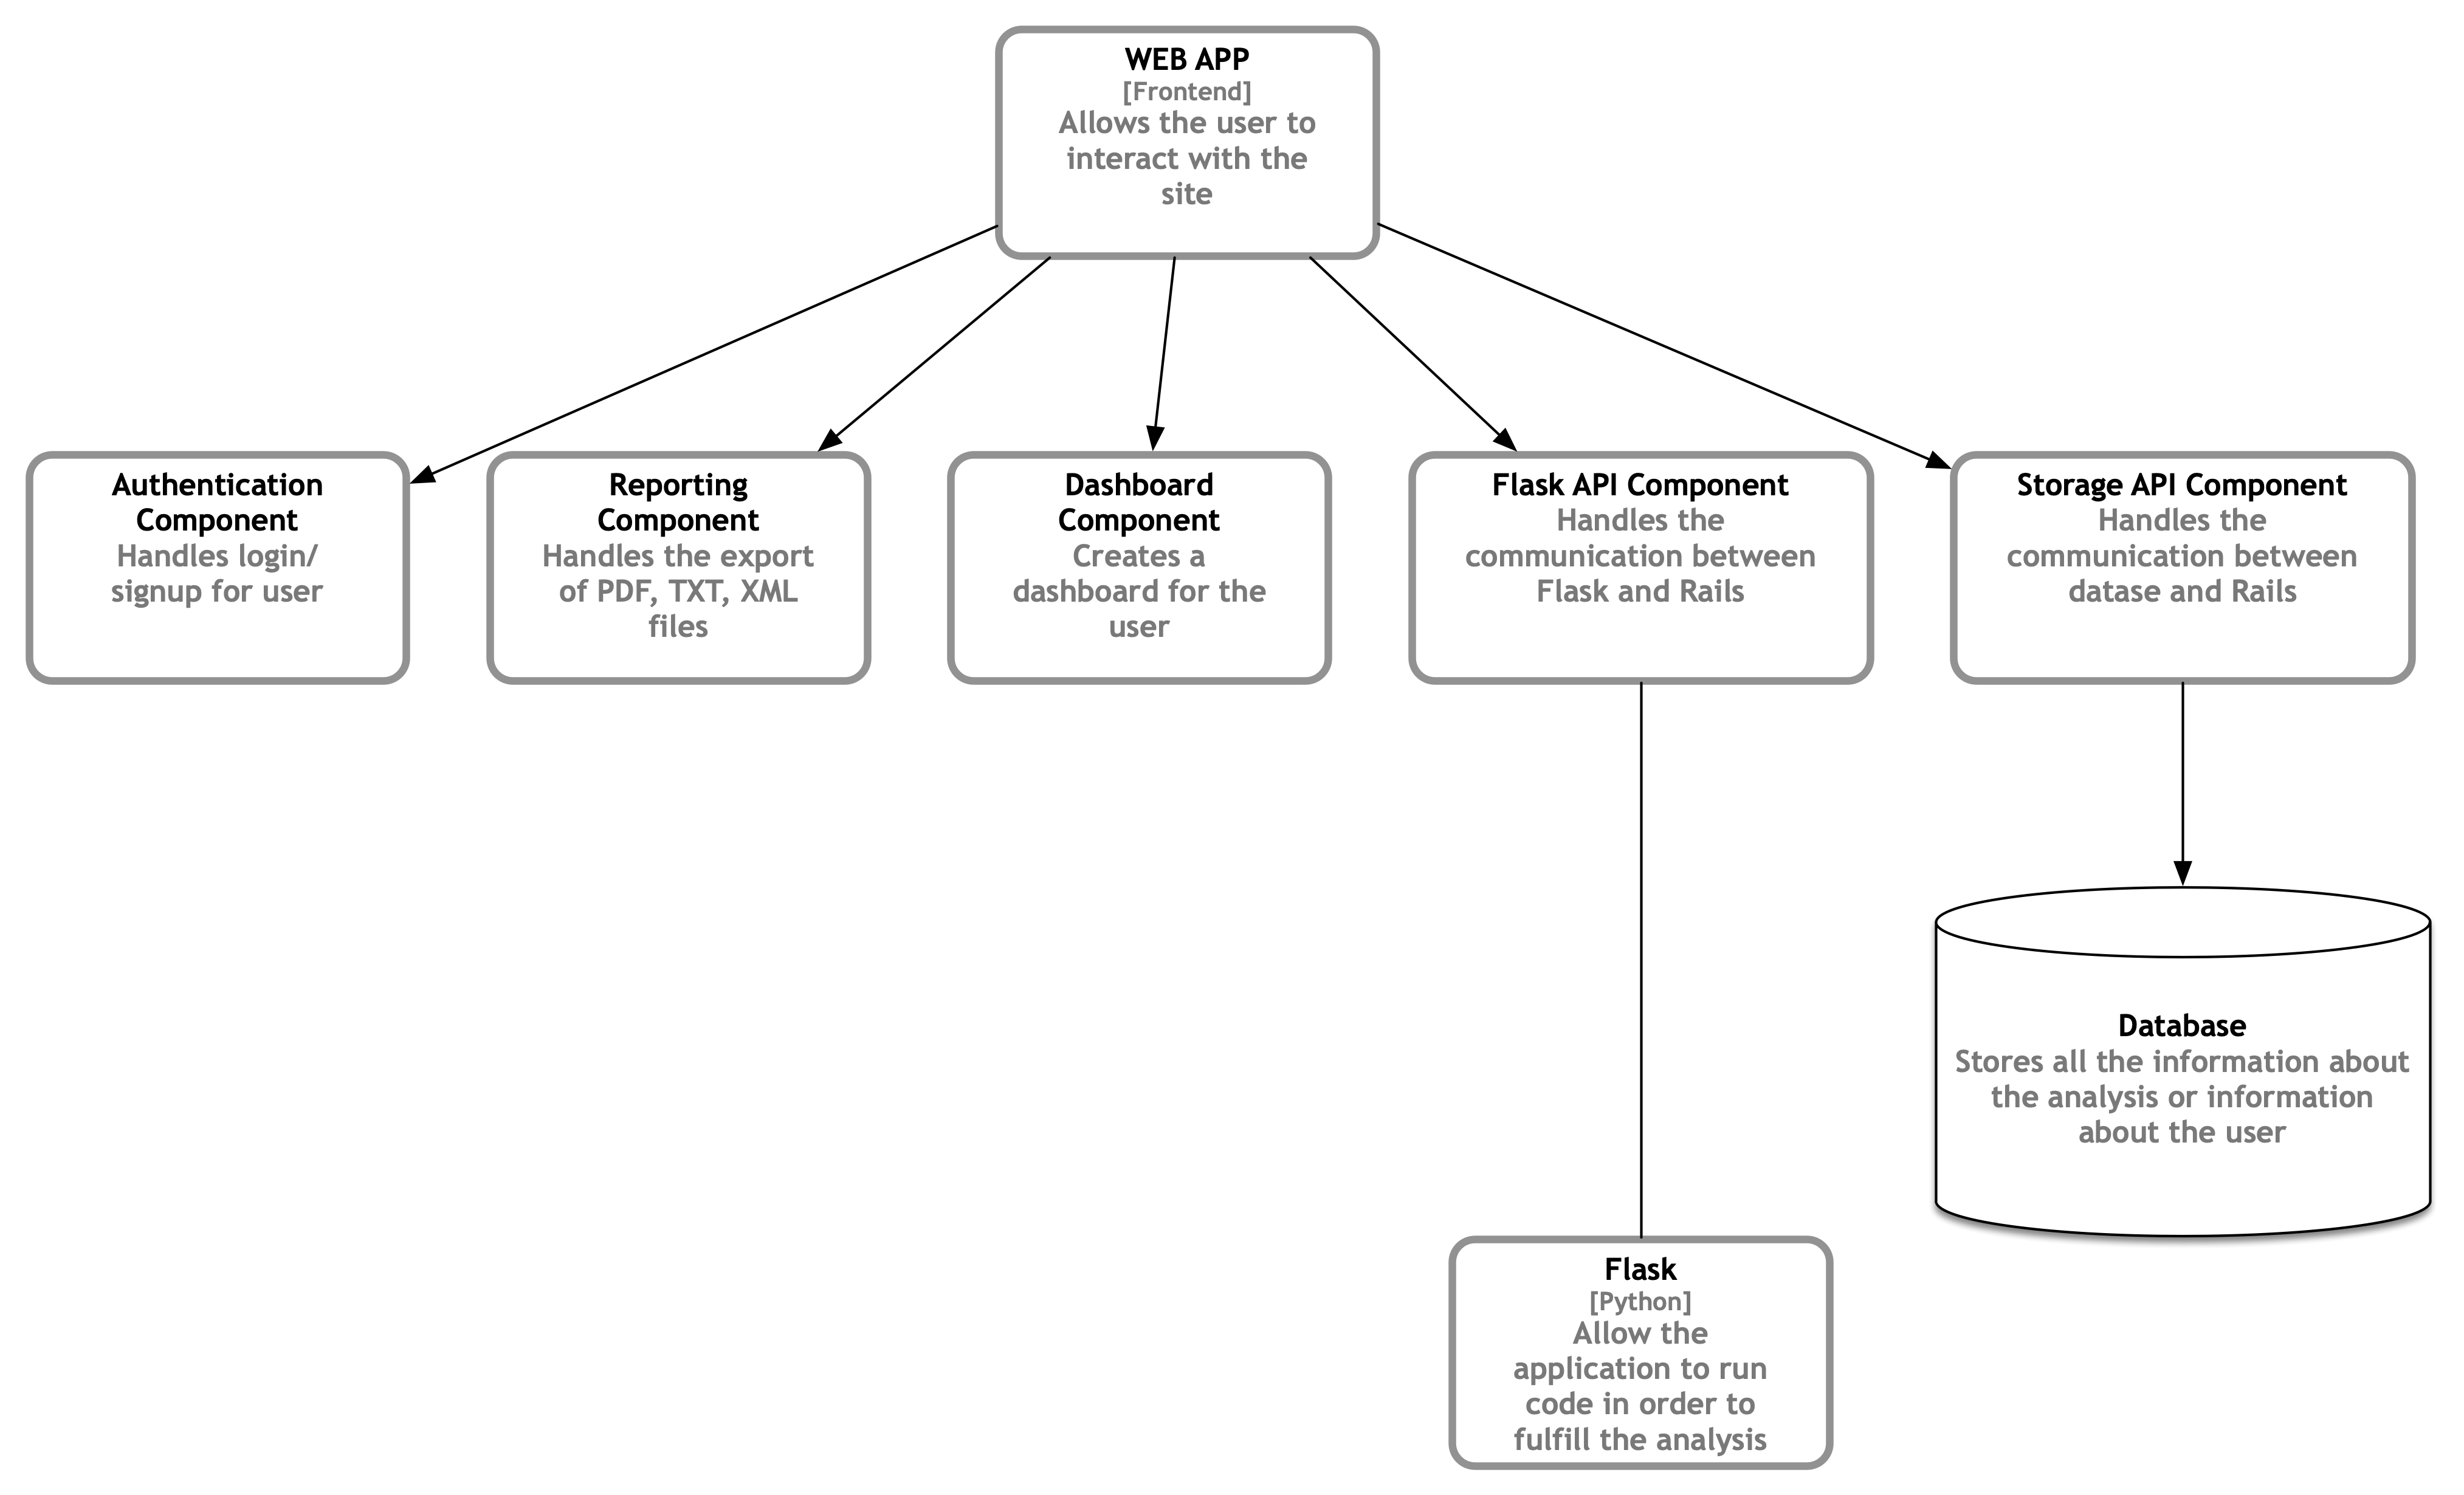
\includegraphics[width=14cm]{img/C43.jpg}
    \caption{Component diagram}
    \label{fig:c42}
\end{figure}

\\
\\
\section{Feature model}

As a second approach, the  Fiure \ref{fig:featureModel} shows the core features of the application, showing which of them are mandatory and which of them are optional.


\clearpage

\afterpage{%
    \clearpage% Flush earlier floats (otherwise order might not be correct)
    \thispagestyle{empty}% empty page style (?)
    \begin{landscape}

\begin{figure}[h!]
    \centering
    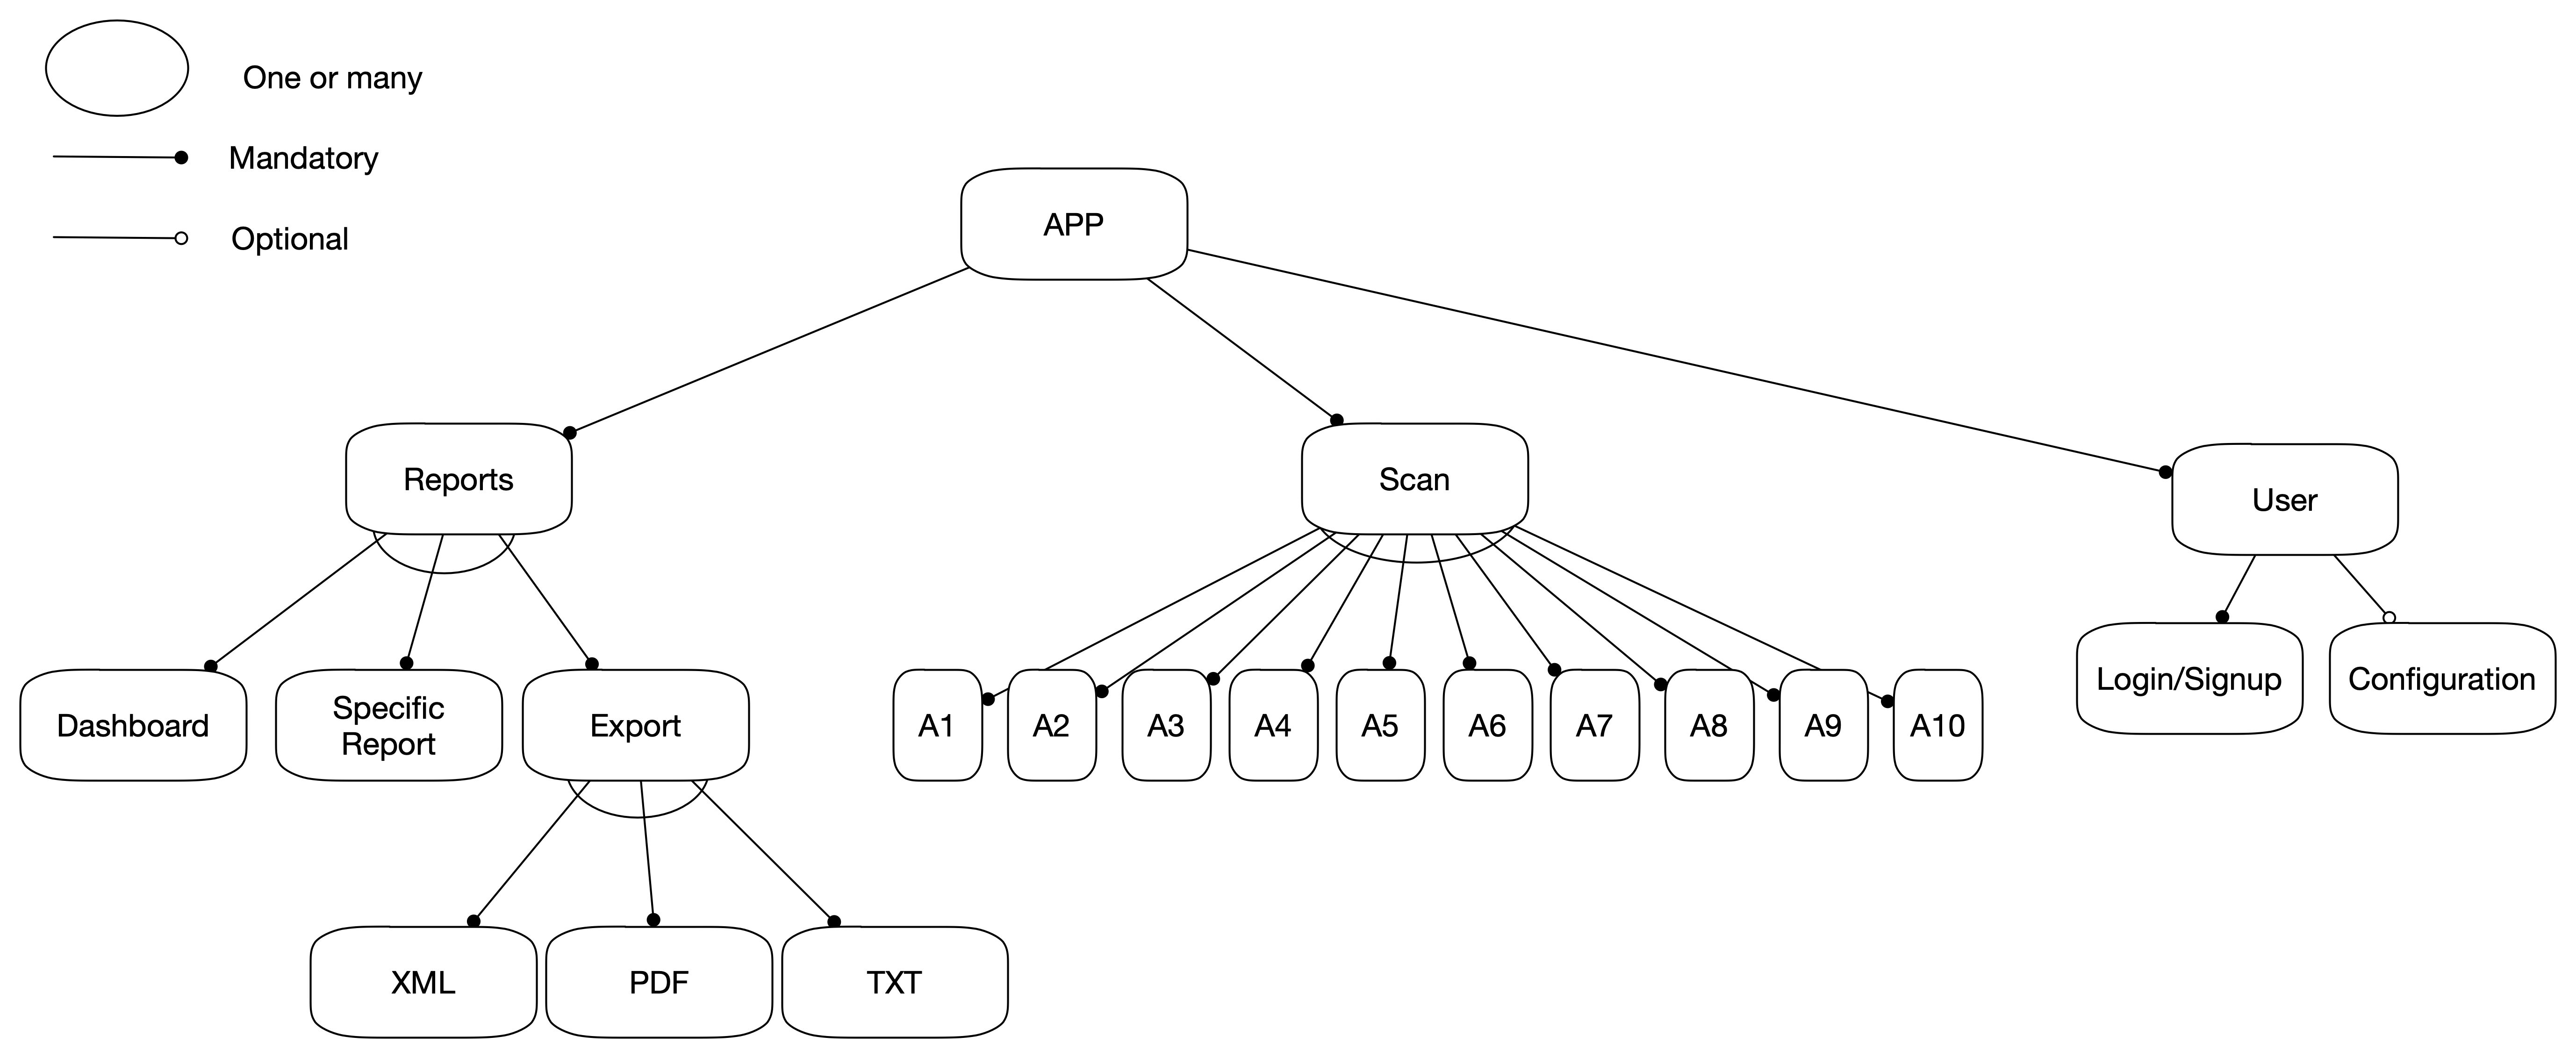
\includegraphics[width=25cm]{img/featureModel.jpg}
    \caption{Feature model}
    \label{fig:featureModel}
\end{figure}


    
    \end{landscape}

    \clearpage% Flush page
}

\clearpage
\section{Squence Diagrams}

In the Figure \ref{fig:urlScan} the sequence between the user's interaction with the web application and all the steps it has to achieve before displaying new information to the user is shown.

\begin{figure}[h!]
    \centering
    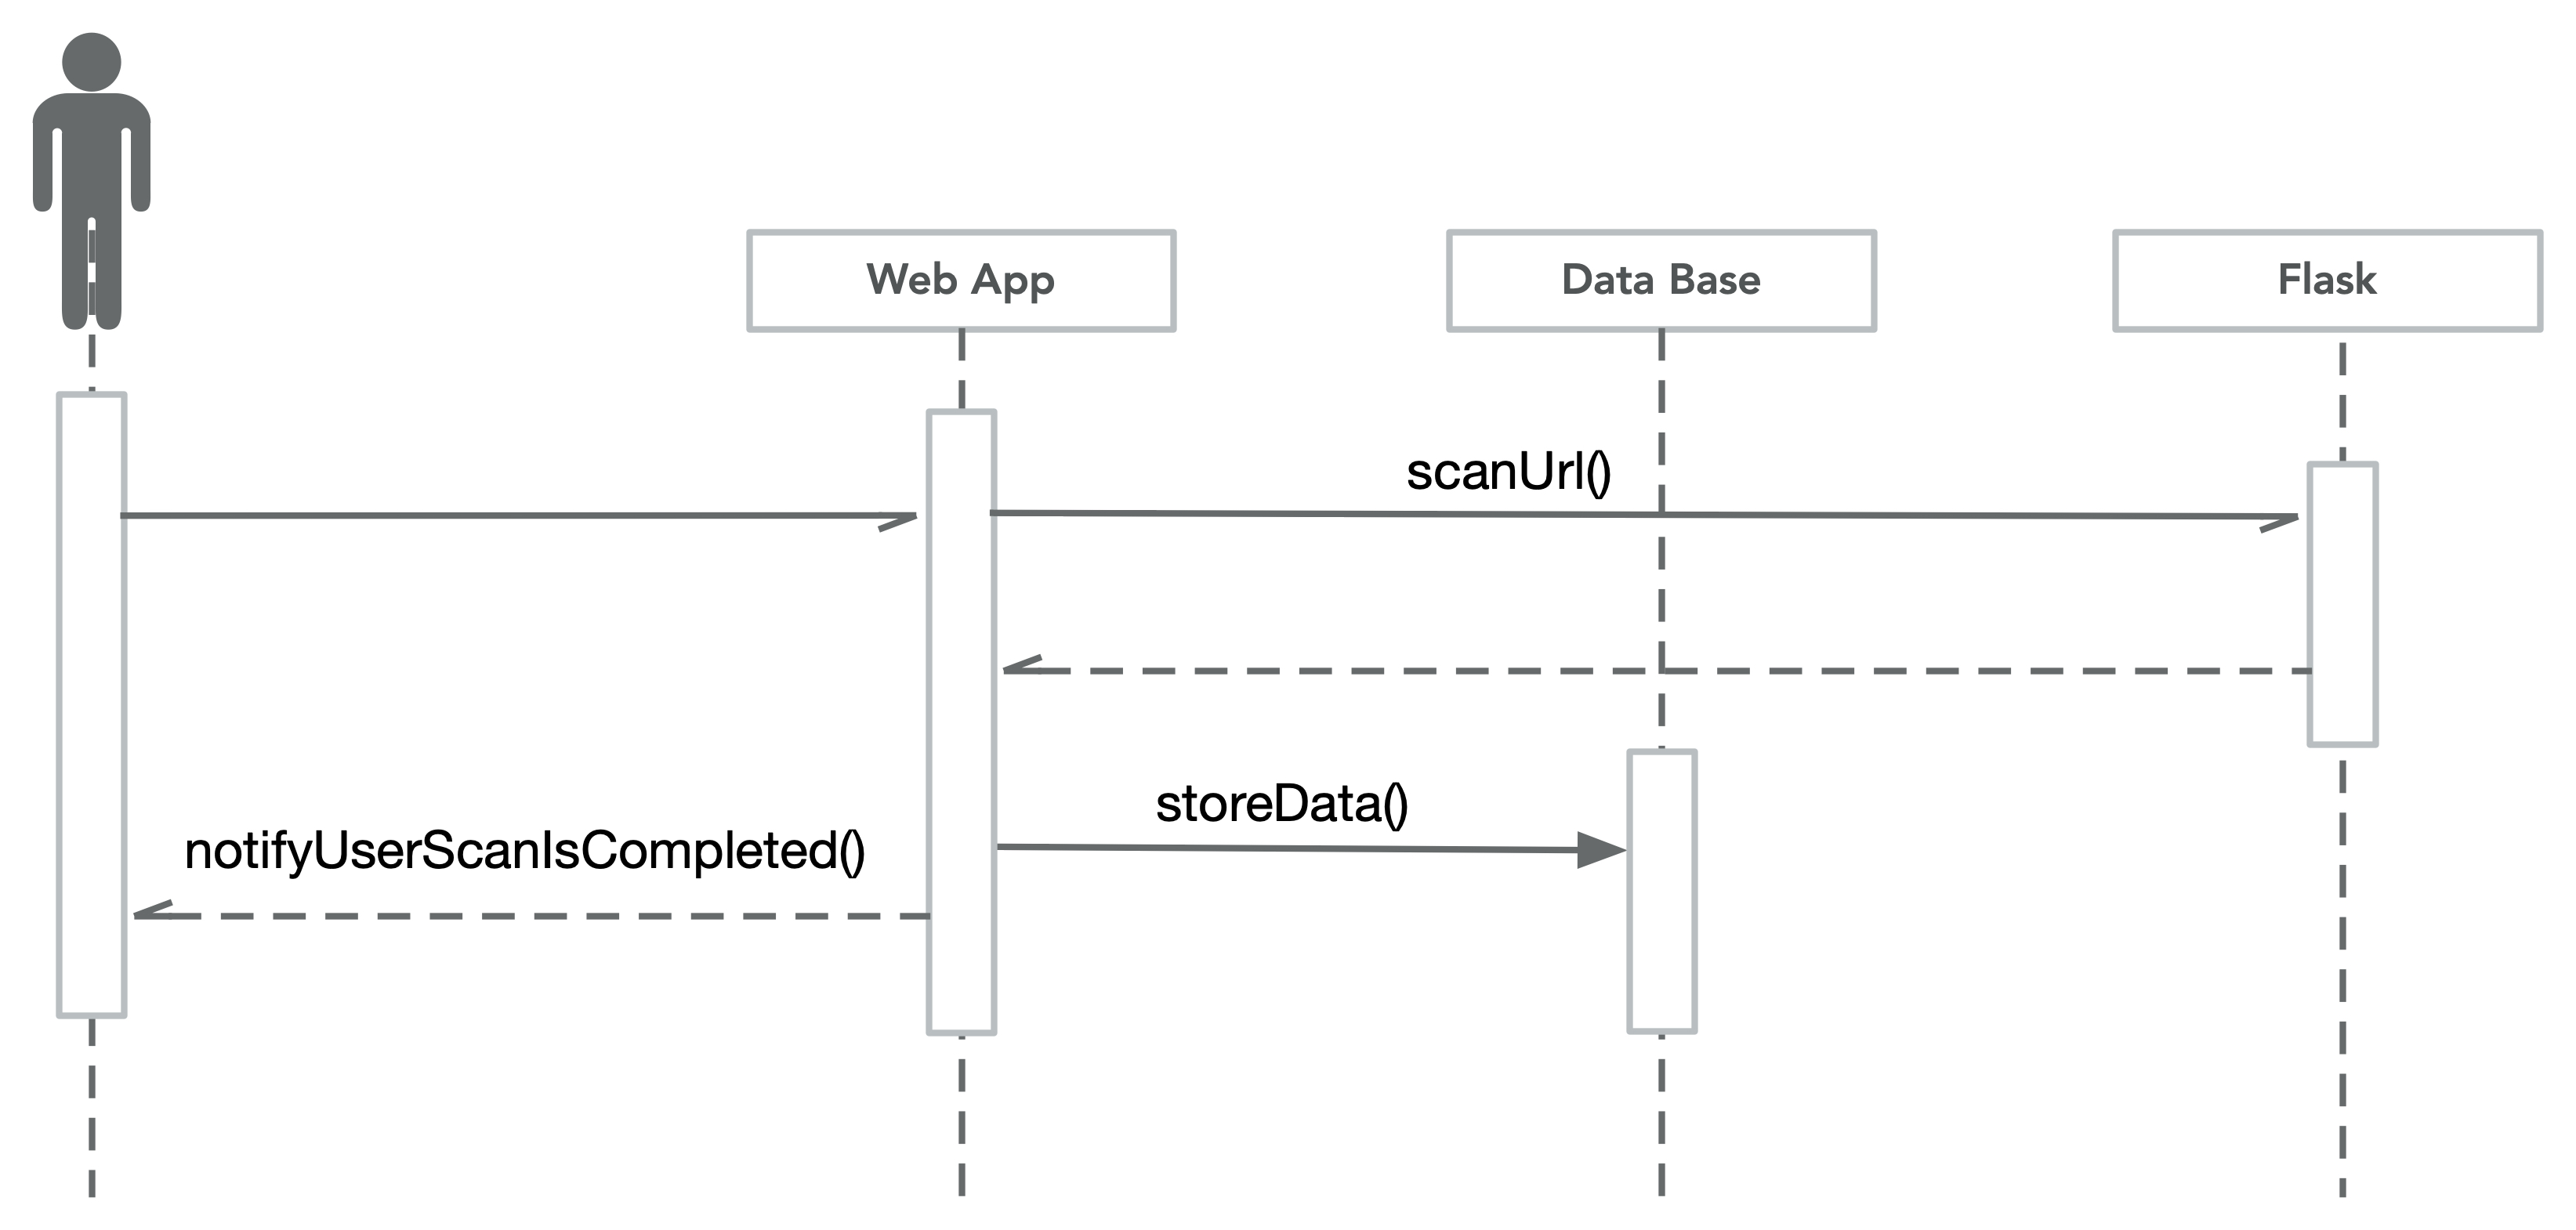
\includegraphics[width=13cm]{img/sequenceScan.jpg}
    \caption{Sequence diagram for scanning a URL}
    \label{fig:urlScan}
\end{figure}

Another important sequence of the application is how the data is displayed on the dashboard as shown on the Figure \ref{fig:dashboard} 

\begin{figure}[h!]
    \centering
    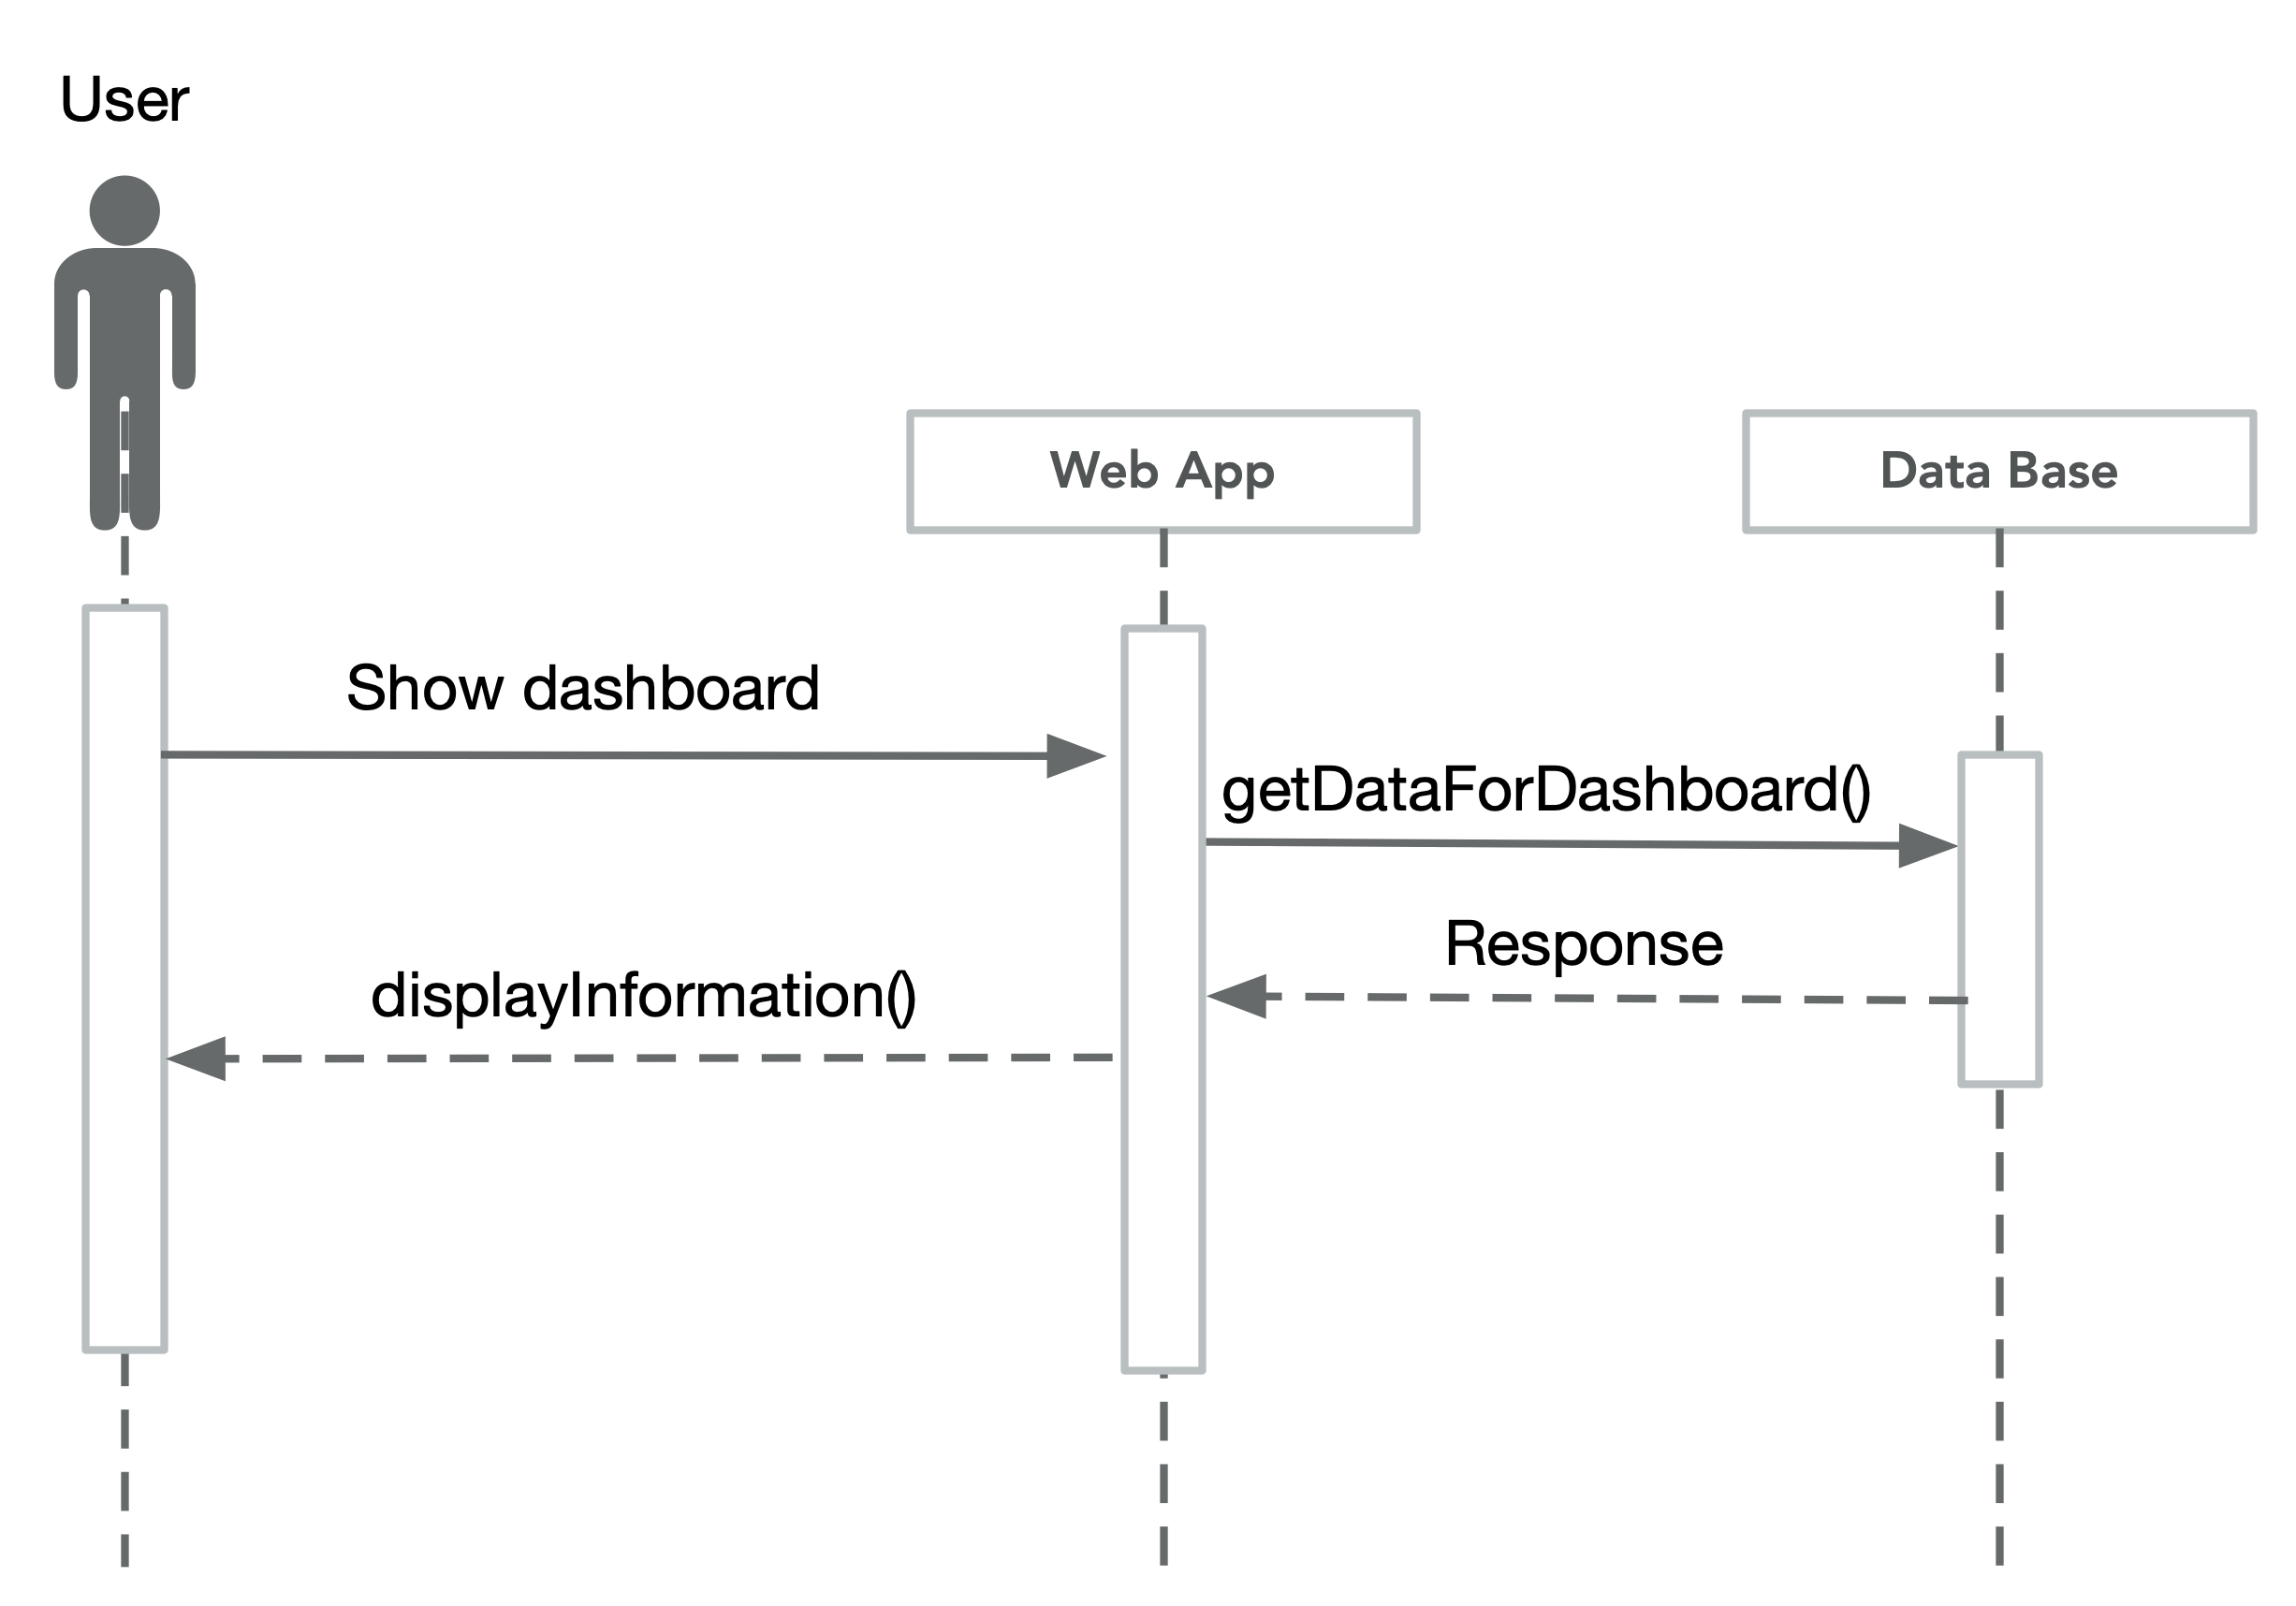
\includegraphics[width=13cm]{img/SequenceDashboard.jpg}
    \caption{Sequence diagram for the dashboard}
    \label{fig:dashboard}
\end{figure}
\section{Database}

As shown on the Figure \ref{fig:database} it can be appreciated that the database consists on 6 tables, each table has a different type of relationship from one another. Most of the relationships shown on the diagram are a one-to-many relationship, there is just one relationship many-to-many between Analyses and Vulnerabilities.

The tables have the following usage/meaning:

\begin{itemize}
    \item Users - stores the user's information.
    \item Analyses - stores each analysis made by a user.
    \item Vulnerabilities - stores the information of the 10 vulnerabilities that can be scanned, each vulnerability is unique so it cannot be repeated.
    \item Analysis-has-Vulnerabilities - it is a relationship between an analysis and all the vulnerabilities that have to be scanned for that specific analysis.
    \item Security-Flaws - stores the data of an specific flaw found on an specific analysis.
    \item Notifications - stores the information of the notifications shown on the site related to a user.
\end{itemize}

\begin{figure}[h!]
    \centering
    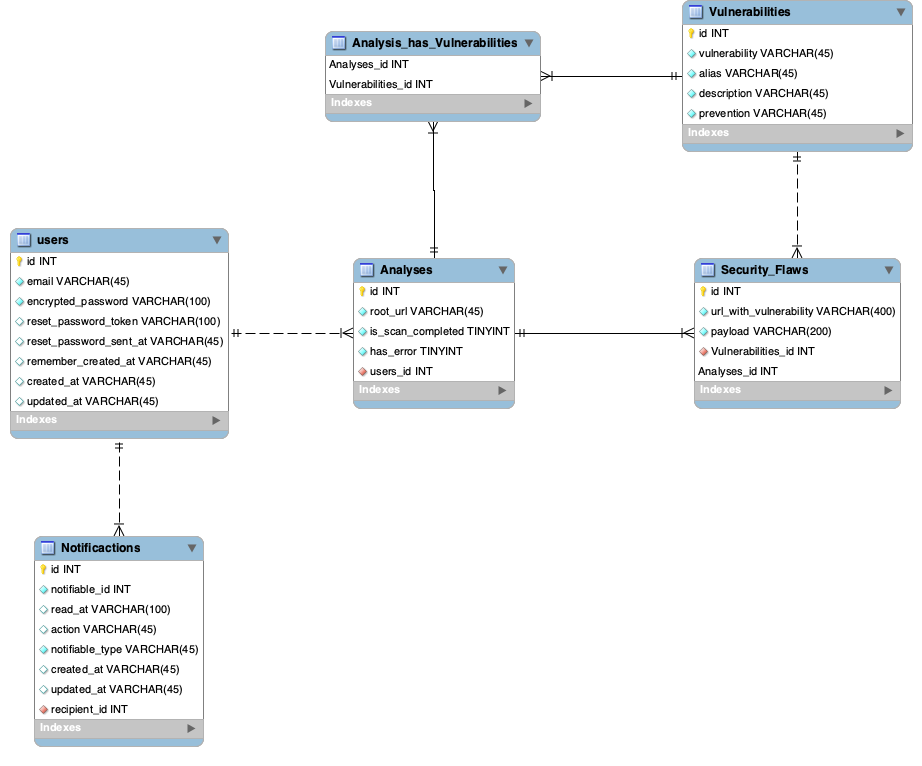
\includegraphics[width=13cm]{img/Databae.png}
    \caption{Relational database's model}
    \label{fig:database}
\end{figure}



\chapter{Possible enhancements for version 2.0}

During the development of the application we noticed that some features could be improved, the following features were considered to be good features for a possible Version 2.0:

\begin{itemize}
    \item Cancel an analysis
    \item Check analysis's status
    \item Show elapsed time of an analysis
    \item Show more statistics or graphics
\end{itemize}

\appendix
\chapter{Appendix}
\renewcommand{\labelenumii}{\theenumii}
\renewcommand{\theenumii}{\theenumi.\arabic{enumii}.}

\section{User Documentation}
Test and manage your Web Applications security with a few clicks, The WASS software allows you to scan a Web Application for security vulnerabilities, save the results of the scan and generate reports in PDF, XML and TXT formats. 

\begin{enumerate}
    \item Create Account
    \begin{enumerate}
    
        \item The first step in order to use WASS is enter to              http://178.128.186.156:3000 in your favorite browser. 
        \begin{figure}[h!]
            \centering
            
\includegraphics[width=14cm]{img/userdoc1.png}
            \caption{WAAS URL}
            \label{fig:wass_url}
        \end{figure}
        
        \item  The next step is to create an user account, navigate to the software and you will see a login page
        \begin{figure}[h!]
            \centering
            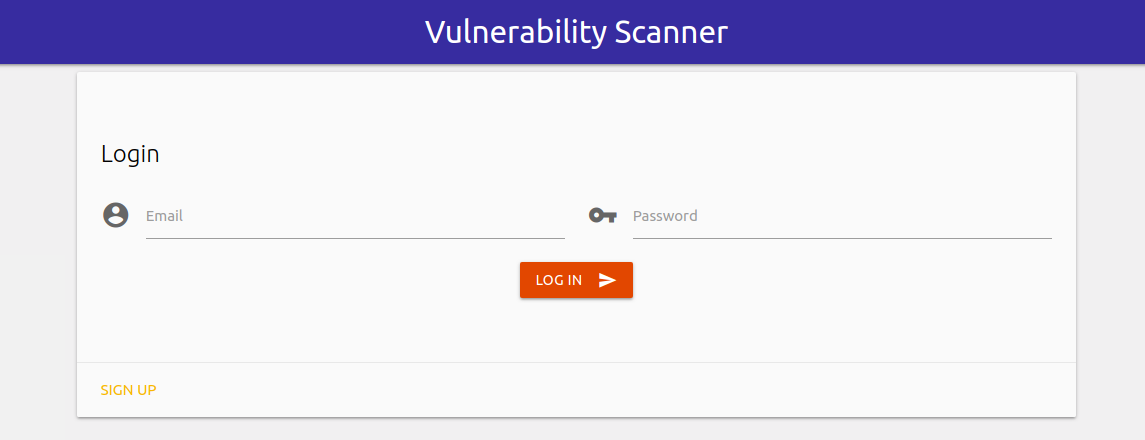
\includegraphics[width=12cm]{img/userdoc2.png}
            \caption{Login page}
            \label{fig:login_page}
        \end{figure}
        
        \item Click on sign up \\
        \begin{figure}[h!]
            \centering
            
\includegraphics[width=14cm]{img/userdoc3.png}
            \caption{Sign up}
            \label{fig:sign_up}
        \end{figure}
        
        \item Insert your email, create a password and click on sign up.
        \begin{figure}[h!]
            \centering
            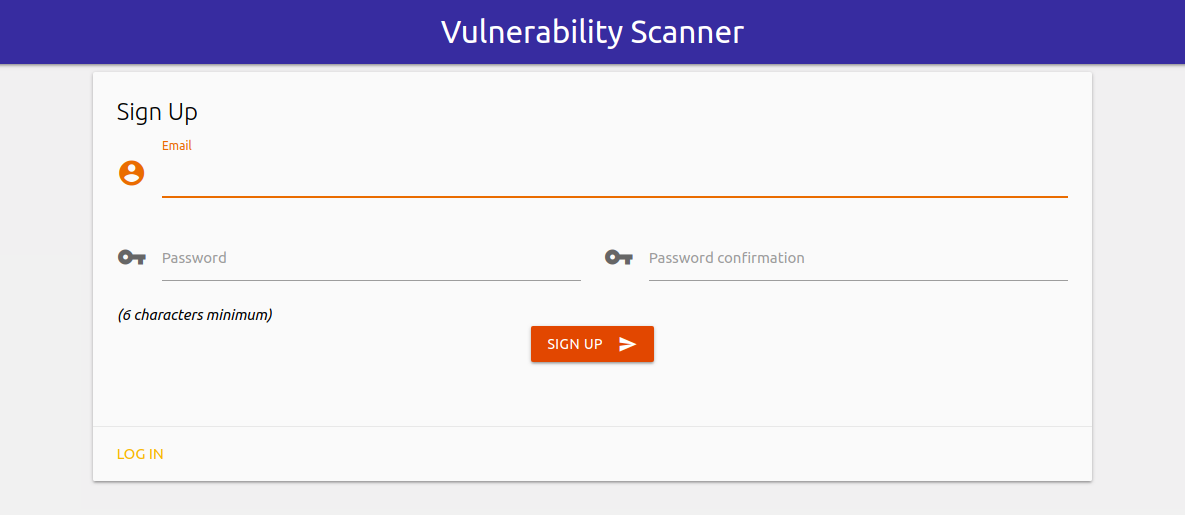
\includegraphics[width=14cm]{img/userdoc4.png}
            \caption{Sign up form}
            \label{fig:sign_up_form}
        \end{figure}
        
      \end{enumerate}
      
      \item Analysing a Web Application by URL 
      \begin{enumerate}
          \item Once you have your user account, login with your email and password and click on log in button.
          \begin{figure}[h!]
            \centering
            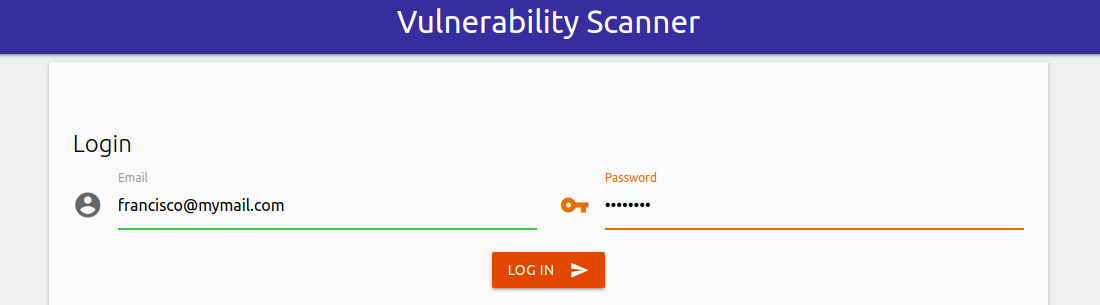
\includegraphics[width=12cm]{img/userdoc5.png}
            \caption{Log in form}
            \label{fig:log_in_form}
          \end{figure} 
          
           \item To analyze a web application, write or paste its URL into the URL field. If the web app you want to scan requires authentication provide the auth token.
           \begin{figure}[h!]
            \centering
            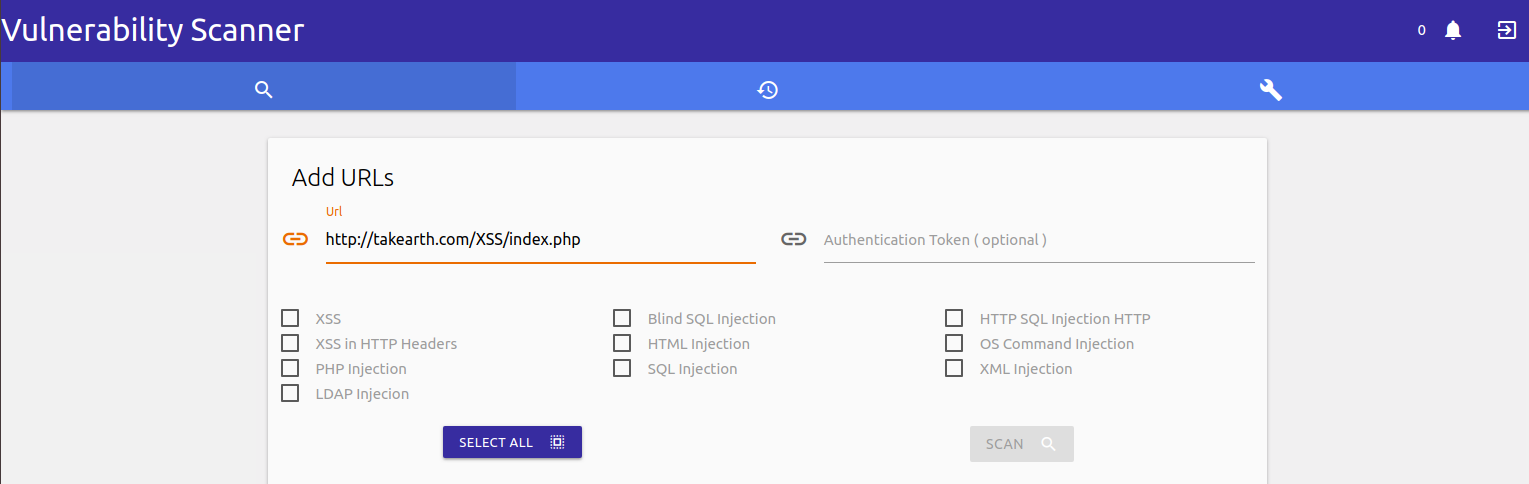
\includegraphics[width=14cm]{img/userdoc6.png}
            \caption{Scanner options}
            \label{fig:scanner_options}
          \end{figure} 
          
          \item Then select the vulnerabilities that you want to analyze and click SCAN \\
          \begin{figure}[h!]
            \centering
            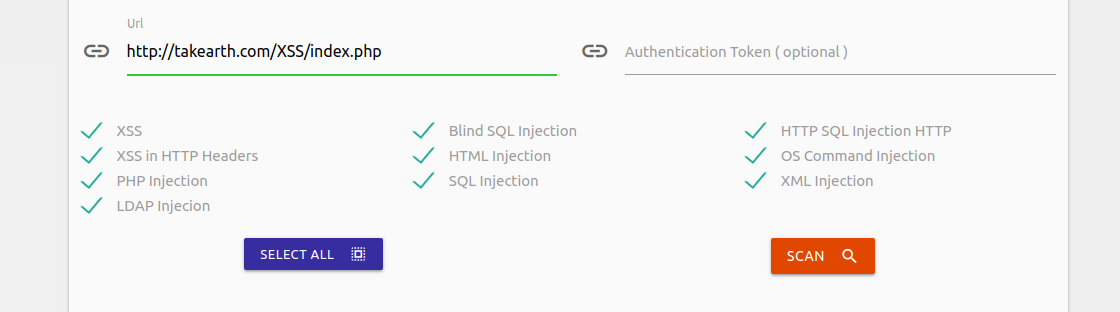
\includegraphics[width=14cm]{img/userdoc7.png}
            \caption{Vulnerabilities selected}
            \label{fig:vulnerabilities_selected}
          \end{figure} \\
          You can click on the select all button to enable all the possible scans\\
          
          \item You will be redirected to the dashboard
          \begin{figure}[h!]
            \centering
            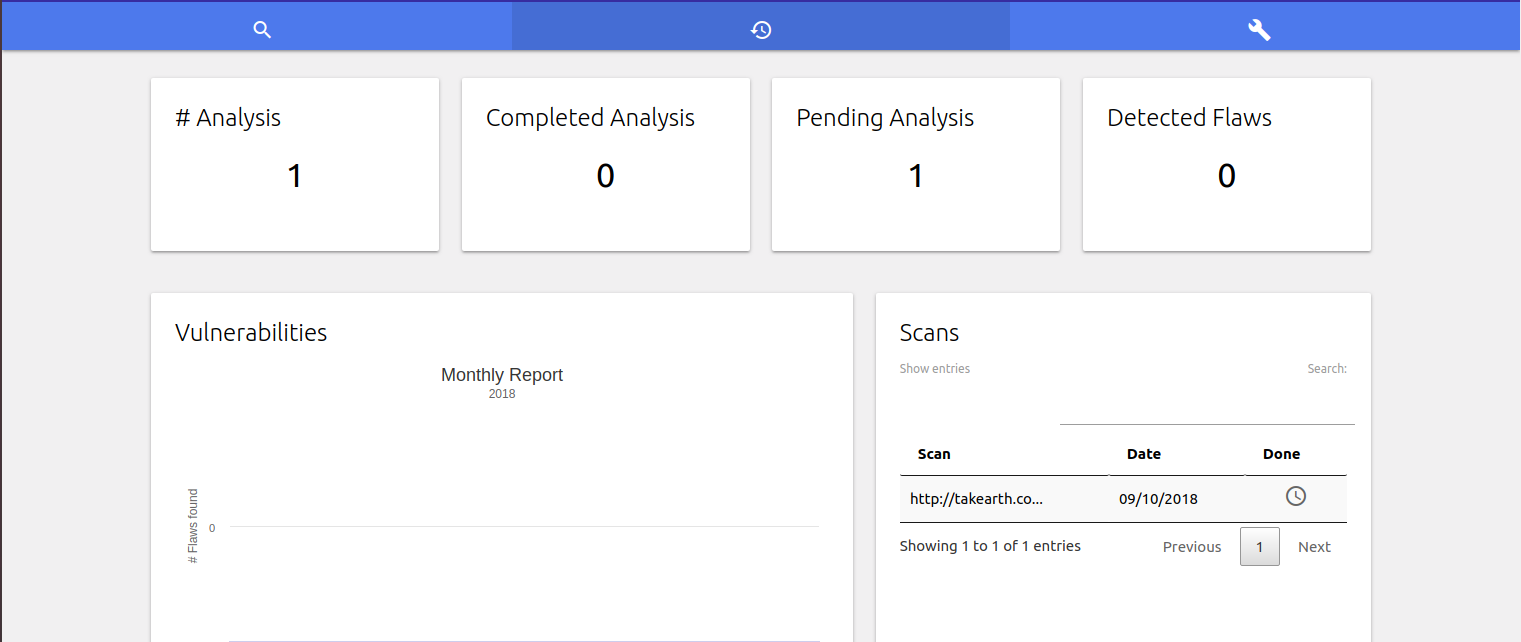
\includegraphics[width=12cm]{img/userdoc8.png}
            \caption{Dashboard}
            \label{fig:dashboard}
          \end{figure}
          
          
      \end{enumerate}
      
      \item Dashboard\\
      Here, you can see the information and results about previous scans.
      \begin{figure}[h!]
        \centering
        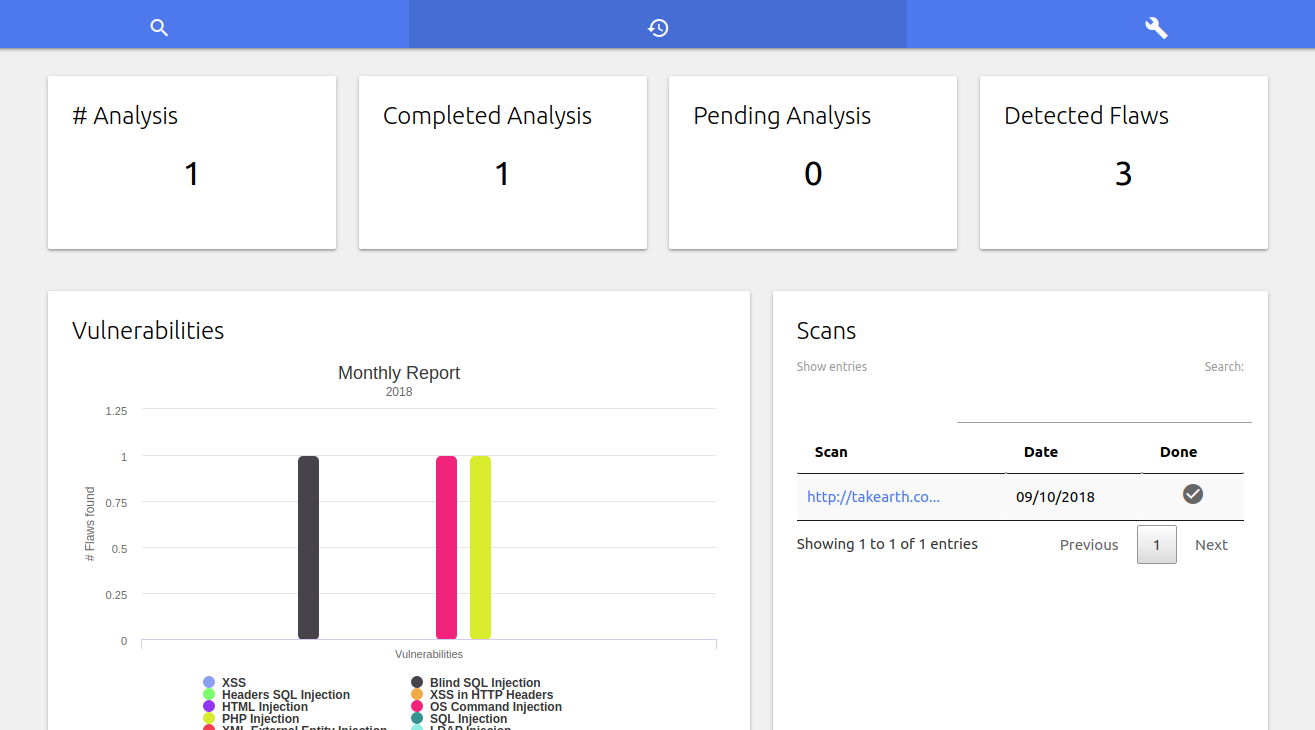
\includegraphics[width=14cm]{img/userdoc9.png}
        \caption{Dashboard}
        \label{fig:dashboard_graphics}
     \end{figure}
     \\
     In this page you can check the total number of analysis, the completed analysis, the pending analysis and the flaws detected.\\
     
     In the right top corner you can see the notifications and the logout buttons 
     \begin{figure}[h!]
        \centering
        
\includegraphics[width=14cm]{img/userdoc10.png}
        \caption{Notifications and log out options}
        \label{fig:notifications_logout}
     \end{figure}
     
     \clearpage
     You can see detailed information of any specific scan by clicking the url in the Recent Scans section \\
     \begin{figure}[h!]
        \centering
        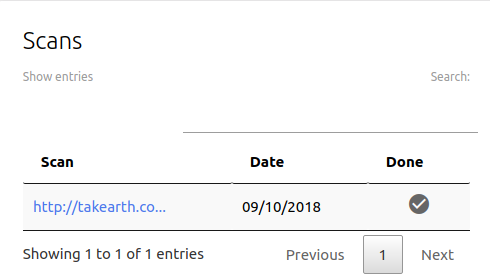
\includegraphics[width=14cm]{img/userdoc11.png}
        \caption{Recent Scans}
        \label{fig:recenly_scanns}
     \end{figure}
     \\
     Here you will see at the left the vulnerabilities found on the analyzed web page, on the right we see a detailed description of the vulnerability
     \begin{figure}[h!]
        \centering
        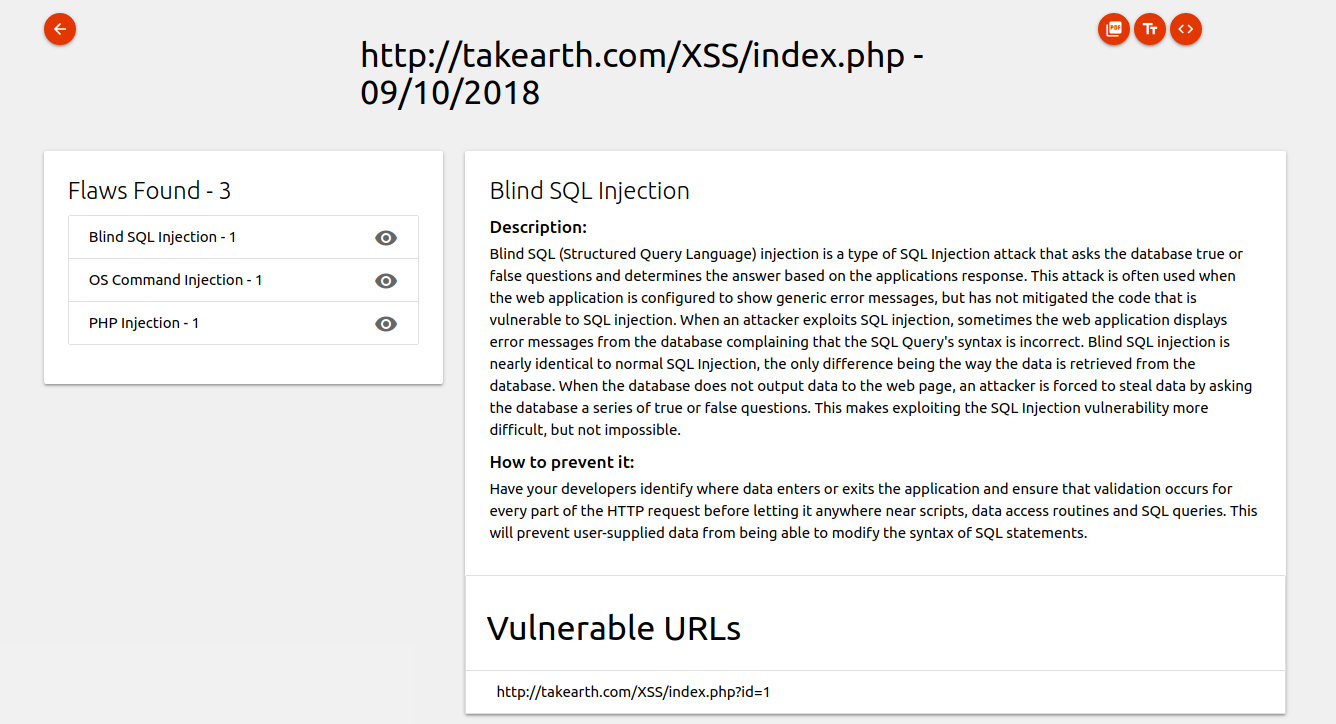
\includegraphics[width=14cm]{img/userdoc12.png}
        \caption{Vulnerabilities details}
        \label{fig:vulnerabilities_details}
     \end{figure}
     \\
     \clearpage
   The number at the right of the flaw represents the number of urls affected by this vulnerability inside the application
   \begin{figure}[h!]
        \centering
        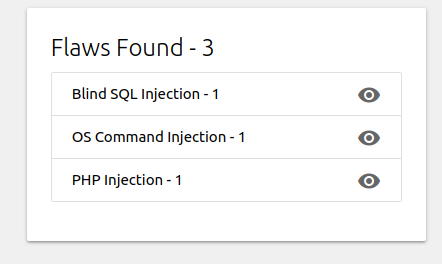
\includegraphics[width=14cm]{img/userdoc13.png}
        \caption{Flaws found}
        \label{fig:flaws_found}
   \end{figure}
   
   \item Exporting reports \\
   You are able to export this analysis in PDF, XML and in plain text or TXT, in order to do this click on the icons on the top right
   \begin{figure}[h!]
        \centering
        
\includegraphics[width=14cm]{img/userdoc14.png}
        \caption{Export icons}
        \label{fig:export_icons}
   \end{figure}
   \clearpage
   When you click on one of the icons a download will start  
   \begin{figure}[h!]
        \centering
        
\includegraphics[width=14cm]{img/userdoc15.png}
        \caption{File Downloaded}
        \label{fig:file_downloaded}
   \end{figure}
   \\
   You should be able to open the file on your prefered reader.
   \begin{figure}[h!]
        \centering
        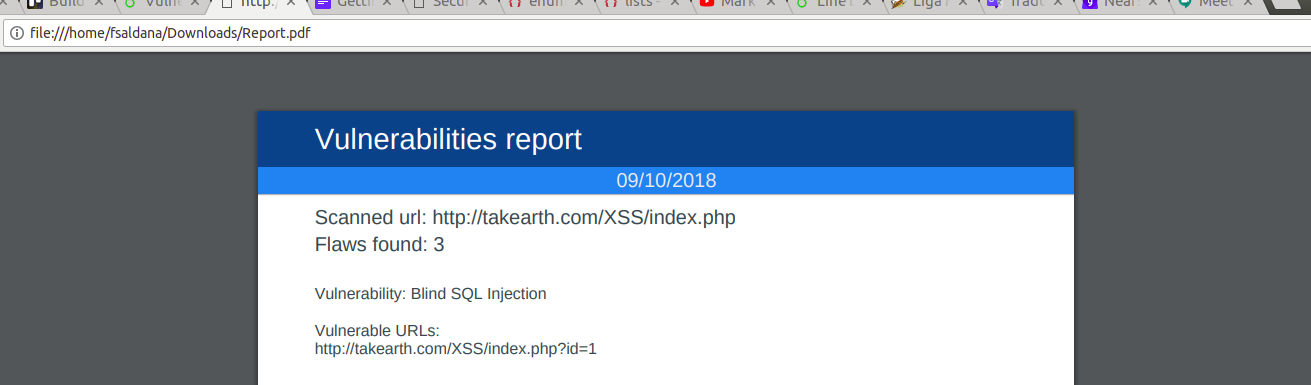
\includegraphics[width=14cm]{img/userdoc16.png}
        \caption{Report}
        \label{fig:report}
   \end{figure}
   
   \item Managing your account \\
   You are able to modify your account email and password, if you want to change one just go to the wrench icon, it's the menu at the right.
   \begin{figure}[h!]
        \centering
        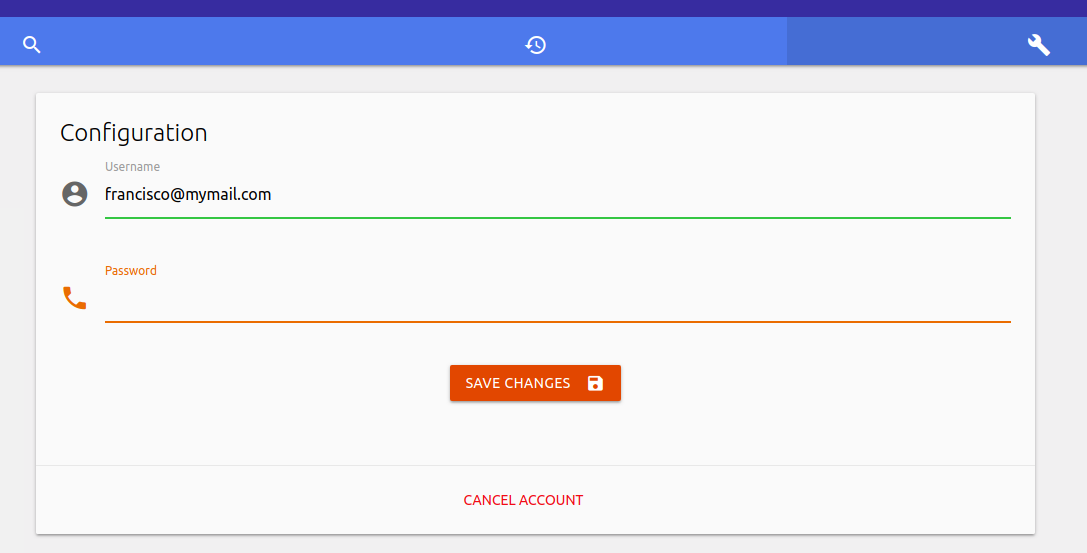
\includegraphics[width=12cm]{img/userdoc17.png}
        \caption{Account configuration}
        \label{fig:account_configuration}
   \end{figure}
   \\
   \\
   Update your credentials and click on SAVE CHANGES in order to conserve the changes, you will be asked to sign up again in order to continue using the scanner.
   \begin{figure}[h!]
        \centering
        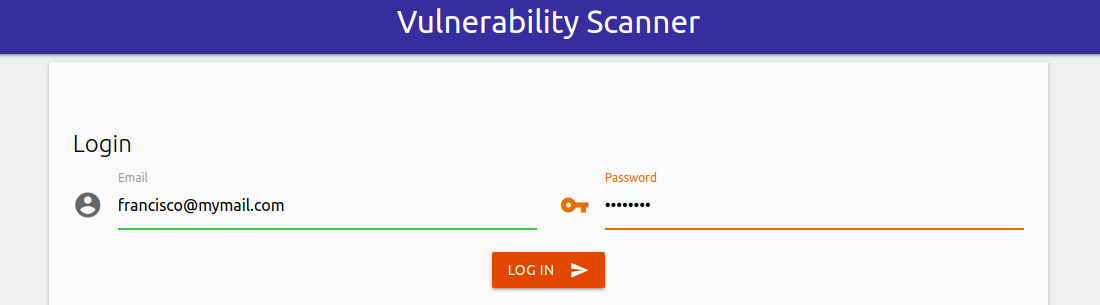
\includegraphics[width=12cm]{img/userdoc5.png}
        \caption{Log in}
        \label{fig:log_in}
   \end{figure}
   
   
   
\end{enumerate}



\clearpage
\section{Developer Documentation}

\subsection{Installing Docker}

Update the apt package index: 
    \begin{minted}{bash}
        $ wget http://tex.stackexchange.com
    \end{minted}

Install packages to allow apt to use repository over HTTPS:
    \begin{minted}{bash}
        $ sudo apt-get install apt-transport-https
        ca-certificates curl software-properties-common
    \end{minted}

Add Docker’s official GPG key
    \begin{minted}{bash}
        $ curl -fsSL https://download.docker.com/linux
        /ubuntu/gpg | sudo apt-key add -
    \end{minted}

Set up the stable repository (copy and paste all line in one go)

    \begin{minted}{bash}
	$ sudo add-apt-repository \
   	"deb [arch=amd64] https://download.docker.com/linux/ubuntu \
        $(lsb_release -cs) \ 
   	stable"
    \end{minted}

Update the apt package index.

    \begin{minted}{bash}
	$ sudo apt-get update
    \end{minted}

Install the latest version of Docker CE

    \begin{minted}{bash}
        $ sudo apt-get install docker-ce
    \end{minted}

Verify that Docker CE is installed correctly by running the hello-world image.
	
	\begin{minted}{bash}
	$ sudo docker run hello world
    \end{minted}
    
Create the docker group.

    \begin{minted}{bash}
	$ sudo groupadd docker
    \end{minted}

Add your user to the docker group.

    \begin{minted}{bash}	
	$ sudo usermod -aG docker $USER
    \end{minted}

Restart the machine 

    \begin{minted}{bash}
	$ sudo reboot
    \end{minted}

Verify that you can run docker commands without sudo

    \begin{minted}{bash}
	$ docker run hello-world
    \end{minted}

Run this command to download the latest version of Docker Compose:

    \begin{minted}{bash}
     $ sudo curl -L "https://github.com/docker/compose/releases
    /download/1.22.0/docker-compose-$(uname -s)-$(uname -m)" -o 
    /usr/local/bin/docker-compose	
    \end{minted}


Apply executable permissions to the binary

    \begin{minted}{bash}
	$ sudo chmod +x /usr/local/bin/docker-compose
    \end{minted}

Test the installation 

    \begin{minted}{bash}
	$ docker-compose --version
    \end{minted}
    
\subsection{Cloning the repositories}

Create a new directory with any name you like

     \begin{minted}{bash}
	$ mkdir VulScanner & cd VulScanner
	\end{minted}

\subsubsection{Cloning and building the python server}

Clone the python server repository inside the folder 
     \begin{minted}{bash}
	$ git clone https://github.com/gmotzespina/VulnerabilityScannerPython
    \end{minted}
    
Move inside the new folder 

     \begin{minted}{bash}
	$ cd VulnerabilityScannerPython
    \end{minted}
    
Run the following command to build the docker image, this is a necessary step in order to run the the ruby client as it depends on this image 
     \begin{minted}{bash}
	$ docker build -t python-scanner . 
    \end{minted}
    
Note that is has a dot at the end

\subsubsection{Cloning the rails app}

Move one directory back and clone the ruby app 
  
  \begin{minted}{bash}
	$ cd ..
	$ git clone https://github.com/gmotzespina/VulnerabilityScanner
   \end{minted}

Move inside the new directory 

  \begin{minted}{bash}
	$ cd VulnerabilityScanner
  \end{minted}

Build the docker image 

  \begin{minted}{bash}
	$ docker-compose build web 
    \end{minted}

Run the rails migrations and database seeding  

  \begin{minted}{bash}
	$ docker-compose run --rm web rails db:create db:migrate
    $ docker-compose run --rm web rake db:seed 
\end{minted}

Run the rails server, this will automatically start the db server and the python server 

  \begin{minted}{bash}
	$ docker-compose up web
   \end{minted}

\subsection{Utilities}
Show mounted images 
    \begin{minted}{bash}
    Docker ps -a 
    \end{minted}








\printbibliography


\end{document}